\documentclass[letterpaper,12pt,oneside]{article}\usepackage[]{graphicx}\usepackage[]{color}
%% maxwidth is the original width if it is less than linewidth
%% otherwise use linewidth (to make sure the graphics do not exceed the margin)
\makeatletter
\def\maxwidth{ %
  \ifdim\Gin@nat@width>\linewidth
    \linewidth
  \else
    \Gin@nat@width
  \fi
}
\makeatother

\definecolor{fgcolor}{rgb}{0.345, 0.345, 0.345}
\newcommand{\hlnum}[1]{\textcolor[rgb]{0.686,0.059,0.569}{#1}}%
\newcommand{\hlstr}[1]{\textcolor[rgb]{0.192,0.494,0.8}{#1}}%
\newcommand{\hlcom}[1]{\textcolor[rgb]{0.678,0.584,0.686}{\textit{#1}}}%
\newcommand{\hlopt}[1]{\textcolor[rgb]{0,0,0}{#1}}%
\newcommand{\hlstd}[1]{\textcolor[rgb]{0.345,0.345,0.345}{#1}}%
\newcommand{\hlkwa}[1]{\textcolor[rgb]{0.161,0.373,0.58}{\textbf{#1}}}%
\newcommand{\hlkwb}[1]{\textcolor[rgb]{0.69,0.353,0.396}{#1}}%
\newcommand{\hlkwc}[1]{\textcolor[rgb]{0.333,0.667,0.333}{#1}}%
\newcommand{\hlkwd}[1]{\textcolor[rgb]{0.737,0.353,0.396}{\textbf{#1}}}%

\usepackage{framed}
\makeatletter
\newenvironment{kframe}{%
 \def\at@end@of@kframe{}%
 \ifinner\ifhmode%
  \def\at@end@of@kframe{\end{minipage}}%
  \begin{minipage}{\columnwidth}%
 \fi\fi%
 \def\FrameCommand##1{\hskip\@totalleftmargin \hskip-\fboxsep
 \colorbox{shadecolor}{##1}\hskip-\fboxsep
     % There is no \\@totalrightmargin, so:
     \hskip-\linewidth \hskip-\@totalleftmargin \hskip\columnwidth}%
 \MakeFramed {\advance\hsize-\width
   \@totalleftmargin\z@ \linewidth\hsize
   \@setminipage}}%
 {\par\unskip\endMakeFramed%
 \at@end@of@kframe}
\makeatother

\definecolor{shadecolor}{rgb}{.97, .97, .97}
\definecolor{messagecolor}{rgb}{0, 0, 0}
\definecolor{warningcolor}{rgb}{1, 0, 1}
\definecolor{errorcolor}{rgb}{1, 0, 0}
\newenvironment{knitrout}{}{} % an empty environment to be redefined in TeX

\usepackage{alltt}
\usepackage[paperwidth=8.5in,paperheight=11in,top=1in,bottom=1in,left=1in,right=1in]{geometry}
\usepackage{setspace}
\usepackage[colorlinks=true,allcolors=Blue]{hyperref}
\usepackage[usenames,dvipsnames]{xcolor}
\usepackage{indentfirst}
\usepackage{titlesec}
\usepackage{multirow}
\usepackage{booktabs}
\usepackage{graphicx}
\usepackage{verbatim}
\usepackage{rotating}
\usepackage{tabularx}
\usepackage{outlines}
\usepackage{lineno}
\usepackage{array}
\usepackage{times}
\usepackage{cleveref}
\usepackage{acronym}
\usepackage[position=t]{subfig}
\usepackage{paralist}
\usepackage[noae]{Sweave}
\usepackage{natbib}
\usepackage{array}
\usepackage{pdflscape}
\usepackage{bm}
\usepackage{amsmath,amsfonts,amssymb,amsthm}
% \usepackage{showlabels}
\bibpunct{(}{)}{,}{a}{}{,}

% page margins and section title formatting
\linespread{1.5}
\setlength{\footskip}{0.5in}
\titleformat*{\section}{\Large\bf\em}
\titleformat*{\subsection}{\singlespace\large\bf}
\titleformat*{\subsubsection}{\singlespace\normalsize\bf\em}
\titlespacing{\section}{0in}{0in}{0in}
\titlespacing{\subsection}{0in}{0in}{0in}
\titlespacing{\subsubsection}{0in}{0in}{0in}

% cleveref options
\crefname{table}{Table}{Tables}
\crefname{figure}{Fig.}{Figs.}
\renewcommand{\figurename}{Fig.}

% aliased citations
\defcitealias{LehrterIR}{Lehrter et al. in review}

%acronyms
\acrodef{cgem}[CGEM]{Coastal Gulf Ecology Model}
\acrodef{gom}[GOM]{Gulf of Mexico}

%for supplemental figures/tables
\newcommand{\beginsupplement}{%
        \setcounter{table}{0}
        \renewcommand{\thetable}{S\arabic{table}}%
        \setcounter{figure}{0}
        \renewcommand{\thefigure}{S\arabic{figure}}%
     }

%knitr options


% get the version based on commit date


% get online bib file


\IfFileExists{upquote.sty}{\usepackage{upquote}}{}
\begin{document}

\raggedbottom
\linenumbers
\raggedright
\urlstyle{same}
\setlength{\parindent}{0.5in}
\renewcommand\refname{References \vspace{12pt}}

\begin{singlespace}
\title{{\bf {\Large Title....}}}
\author{
  {\bf {\normalsize Marcus W. Beck$^1$, John C. Lehrter$^1$}}
  \\\\{\textit {\normalsize $^1$USEPA National Health and Environmental Effects Research Laboratory}}
  \\{\textit {\normalsize Gulf Ecology Division, 1 Sabine Island Drive, Gulf Breeze, FL 32561}}
	\\{\textit {\normalsize Phone: 850-934-2480, Fax: 850-934-2401}}
	\\{\textit {\normalsize Emails: \href{mailto:beck.marcus@epa.gov}{beck.marcus@epa.gov}, \href{mailto:lehrter.john@epa.gov}{lehrter.john@epa.gov}}}
  \vspace{1in} 
  \\ Version Date:   Mon Jun 13 10:12:26 2016 -0500
	}
\date{}
\maketitle
\end{singlespace}
\clearpage

\begin{abstract}
\noindent Bio-geo-chemical models are useful tools in environmental sciences that can guide management and policy-making. Consequently, significant time and resources are spent developing these models in system-specific contexts. The optimization of model parameters to maximize precision, including transferability of these models to different systems, are fundamental concerns in the development and application of these tools. This study describes quantitative limitations of coupled hydrodynamic-ecological modelling by contrasting numeric and ecological certainty with a systematic framework for characterizing parameter sensitivity and identifability.  We evaluate a simple bio-geo-chemical model that is the 1-dimensional unit of a larger spatio-temporal model of hypoxia on the Louisiana Shelf of Gulf of Mexico as an example. Results from analysis of the 1D model are used to infer larger trends in dissolved oxygen dynamics over time, having implications for understanding factors that contribute to environmental conditions that are detrimental to aquatic resources.  In particular, we focus on issues of parameter identifiability using local sensitivity analyses to provide quantitative descriptions of numerical constraints on model precision.  We argue that quantitative and ecological certainty in model calibration are often at odds and the practitioner must explicitly choose model components to optimize given tradeoffs between the two. We further conclude that numerically optimal parameter sets for models of hypoxia are often small subsets of the complete parameter set because of redundancies in the unique effects of paramater perturbations on model output.  As a result, we demonstrate that use of a model for inference into ecological mechanisms of observed or predicted changes in hypoxic condition can be potentially misguided in the absence of quantitative descriptions of identifiability.  Although these concerns have been expressed in the literature, they are rarely explicitly addressed or included in model evaluations.  In addition to immediate implications for regional models, we provide a framework for describing the effects of parameter uncertainty and identifiability that can be applied to similar models to better inform environmental management.
\end{abstract}
\acresetall

\section{Introduction}

\begin{enumerate}
\item Simulation/biogeochemical/process-based models overview, contrast with statistical models
\item What models seek to provide - generality, precision, realism \cite{Levins66}, there is a tradeoff so models are 1) developed in partial independence and dependence on the world and theory, 2) function autonomously from both, or 3) represent both at the same time, from \cite{Morrison99}, cited in \cite{Ganju16}.  This is similar to the bias-variance tradeoff for statistical models, e.g., overparameterization of a model makes it very biased as it fits the data (the world) exactly, tradeoff between sensitity and error with changes in model complexity (more complexity is less error but increasing sensitivity) described in \cite{Snowling01}
\item How is model performance/uncertainty evaluated regarding what they should provide - structural, observational, parameter \cite{Beck87}?
\item Parameter uncertainy as low-hanging fruit - can do post-hoc and from inner to outer level of complexity, parameter uncertainty is the most common, e.g., marine ecological model \cite{Mateus15}, but stopped short, global sensitivity analysis of eutrophication model \cite{Estrada10}
\item Challenges related to uncertainty - similar to degrees of freedom, identifiability definition from \cite{Brun01} and need to evaluate identifiability \cite{Fasham06}, \cite{Omlin01} did a similar analysis with freshwater biogeochem model
\end{enumerate}

This study describes a parameter sensitivity analysis to evaluate identifiability for a bio-geo-chemical model of hypoxia for the northern \ac{gom}.  We evaluate a simple 1-dimensional unit of a larger spatial-temporal model to explore relationships between multiple parameter sets and hypoxia dynamics on the Lousiana coastal shelf.  The study also provides a general framework for sensitivity analysis and parameter identifiability that can be used on similar mechanistic models.  Specifically, an assumption is that models are generally over-parameterized and only a finite and smaller subset of the larger parameter set can be optimized for a given research question or dataset.  We provide explicit guidance for choosing such subsets of the parameter space given constraints on identifiability as directly related to sensitivity analyses.  The specific objectives are to \begin{inparaenum}[1\upshape)]
\item identify the parameters that have the greatest influence on dissolved oxygen using local sensitivity analysis,
\item quantify the identifiability of subsets of the total parameter space based on sensitivity,
\item provide a set of heuristics for choosing parameters based on sensitivity and parameter categories with the larger mechanistic model, including extension to other state variables, and 
\item discuss implications for hypoxia formation in coastal regions, including management strategies for nutrient reduction and use of mechanistic models to inform decision-making.
\end{inparaenum}
The `optimum' parameter space is defined as the chosen subset that represents the maximum number of identifiable parameters.  Here, `optimum' is both a qualitative description based on a research question or management goal and a quantitative objective based on numerical optimization criteria for fitting model output to a calibration dataset.  These results can be used to refine existing models or guide application of models to novel contexts, such as downscaling or application to new environments. 

\section{Methods}

\subsection{Model description}

Three-dimensional numerical models have recently been developed for the northern \ac{gom} to explore dynamics in bottom-water hypoxia and primary production (\citealt{Fennel13,Pauer16}, \citetalias{LehrterIR}).  The Louisiana coastal shelf  covers an area of  


CGEM \citepalias{LehrterIR}, FishTank, parameters and parameter categories, how they compare to other models

\subsection{Local sensitivity analysis}

Methods from \cite{Reichert01,Soetaert10}

Sensitivity of the model to parameter changes is evaluated using the difference in model results before and after perturbing each parameter value.  Each parameter is perturbed by the same value as a percentage of the whole.  The default value (as 1 + 1e-8 proportion, default value for `tiny` argument in `sensFun`).  A sensitivity value $S$ is estimated for each time step $i$ given a set value for parameter $j$ as:

\begin{equation}
S_{ij} = \frac{\partial y_i}{\partial \Theta_j}\cdot\frac{w_{\Theta_j}}{w_{y_i}}
\end{equation}

where the estimate depends on the change in the predicted value for response variable $y$ divided by the change in the parameter $\Theta_j$ multiplied by the quotient of scaling factors $w$ for each.  The scaling factors, $w_{\Theta_j}$ for the parameter $\Theta_j$ and $w_{y_i}$ for response variable $y$, are set as the default value of the unperturbed parameter and the predicted value of $y_i$ after perturbation \citep{Soetaert10}.  The scaling ensures the estimates are unitless such that the relative magnitudes provide a comparison for model sensitivity to parameter changes that may vary in scale.  The FME package summarizes sensitivity as $L1$ and $L2$ across the time series:

\begin{equation}
L1 = \sum|S_{ij}|/n
\end{equation}
\begin{equation}
L2 = \sqrt{\sum\left(S_{ij}^2\right)|/n}
\end{equation}

The mean, minimum, and maximum $S_{ij}$ values for each parameter are also reported.  In general, positive mean sensitivity estimates generally indicate that a parameter has a positive effect on the model results for a given increase in the parameter.  However, the effect can change over time so a plot of the 'sensitivity function' should be viewed which shows the difference from the values of the response variable before and after changing a parameter value.  Note that the perturbation factor in `sensFun` depends on the default value of each parameter such perturbations are not consistent for parameter values less than or greater than the perturbation factor.  This can produce results that are inconsistent for different levels of perturbation.  A custom function was keeps the perturbation factors constant regardless of the magnitude of the default values.  Sensitiviy for each parameter using the custom function are estimated using the above equations from the FME package. All parameters that are considered 'sensitive' should be further evaluated by plotting the predictions before and after perturbation and across the total range of the parameter. 

Each parameter was perturbed by 50\% using `sensfun` to identify model sensitivity.  Parameters that produced different model results from the default values are shown below, by category. 

The parameters that have the greatest effect on the model by category (optics, organics, phytoplankton, zooplankton) are as follows.

Plotting the raw values from the sensitivity analysis provides a visual assessment of changes.

\subsection{Identifiability}

Identifiability describes the ability to estimate a parameter in relation to variation among the remaining parameters.  A parameter is identifiable if all parameters within the set can be uniquely estimated based on the observed data.  Parameters that are unidentifiable typically produce similar model outputs for a given relative perturbation, i.e., the effect of altering one parameter can be undone by altering one or more other parameters.  Model calibration will not converge for parameters sets that are unidentifiable.  Identifiability is estimated from the minimum eigenvector of the cross-product of a model's sensitivity matrix \citep{Brun01,Omlin01}:

\begin{equation}
\gamma = \frac{1} {\sqrt{ \min \left(\rm{EV}[\hat{S}^\intercal \hat{S}]\right)}}
\end{equation}

where $\gamma$ ranges from one to infinity for perfectly identifiable (orthogonal) or unidentifiable (perfectly collinear) results for a set of parameters in the sensitivity matrix $S$.  Identifiability can be estimated for any combination of parameters for a model.  Values less than 10-15 indicate parameters are generally identifiable.  The FME package provides the `collin` function to estimate identifiability of output from the `sensFun`.  For reasons described above, a custom function was created to determine identifiability from model residuals, where the residauls were based on a relative perturbation of the model parameters.  A comparison of results of identifiability using the custom functions and those from the FME package were generally in agreement.  Standard output from the identifiability function is shown below, where identifiability is displayed as a matrix with increasing combinations of subsets of the parameters.    



The identifiability functions evaluate the ability to identify all subsets from pairwise to all parameters in the subset.  As an example, the identifiability of pairwise combinations for each of the categories are shown below.



Pairwise identifiability of the top two most sensitive parameters in each category is shown, first as a table showing all unique combinations from two to all parameters and second as a figure showing pairwise combinations.

\subsection{Identifying subsets and testing calibration}

Model calibration must consider the competing objectives of parameter inclusion and identifability.  Estimating parameters for novel datasets increases model complexity and the ability to identify parameters decreases with the inclusion of parameters to estimate.  The above analyses indicated that estimating all of the parameters was impossible because of redundancies in the the model output.  Calibration to novel datasets should balance the competing objectives of identifiability while including parameters for which model output is most sensitive.  The plots below show different scenarios of parameter inclusion for model calibration.  Reading each plot from left to right can be interpreted as including additional parameters, where each parameter is ranked by relative sensitivity.  The inset in each plot shows the identifiability of including parameters, up to a maximum where additional inclusion exceeds the identifability threshold of fifteen.  The scenarios for including parameters all begin with the parameters that have the greatest effect on the model output.  The inclusion of additional parameters depends on the scenario.  The first scenario selected parameters by decreasing sensitivity within each category (i.e., four separate models calibrated for optics, organics, phytoplankton, or zooplankton), the second scenario selected parameters by sensitivity regardless of category, and the third scenario selects parameters by sensitivity with equal representation between categories.  Boxes in each plot represent a unique parameter and the numbers in each box represent the relative rank of a parameter's sensitivity to the model output within each category. 

The following plots show identifiability with the addition of parameters. 


\section{Results}

\section{Discussion}

Questions specific to GOM - what initial conditions are important? How many phytoplankton groups do we need (e.g., related to structural uncertainty)?

How does the assimilation of additional parameters (e.g., other state variables) during calibration influence the conclusions?

How does uncertainty translate to what a model should provide (generality v precision)?  The first step - find out what can be optimized but then do not overfit....

What about structural uncertainty - does sensitivity of a model to variation in a parameter imply parameter uncertainty and/or structural uncertainty?

A final point about optimization with identifiable parameter sets - optimization to fit the data still does not ensure a correct model.  Failing in one way can be over-compensated by another feature, e.g., the parameter set that is optimized (see \cite{Flynn05}, p. 1207, third paragraph)

\cite{Omlin01} state that the sensitivity, identifiability, estimation process is iterative (p. 113), need to rinse and repeat for proper calibration. 

How to improve identifiability - get more/better observed data, include obs from other state variables in RSS minimization (eqn q in \cite{Omlin01})

Alternative methods for uncertainty analysis - bayesian, MCMC, nonlinear calibration-constrained optimization \citep{Gallagher07}

\clearpage
\begin{singlespace}
\bibliographystyle{apalike_mine}
\bibliography{refs}
\end{singlespace}
\clearpage

%%%%%%
% figures
\begin{figure}[!ht]

{\centering 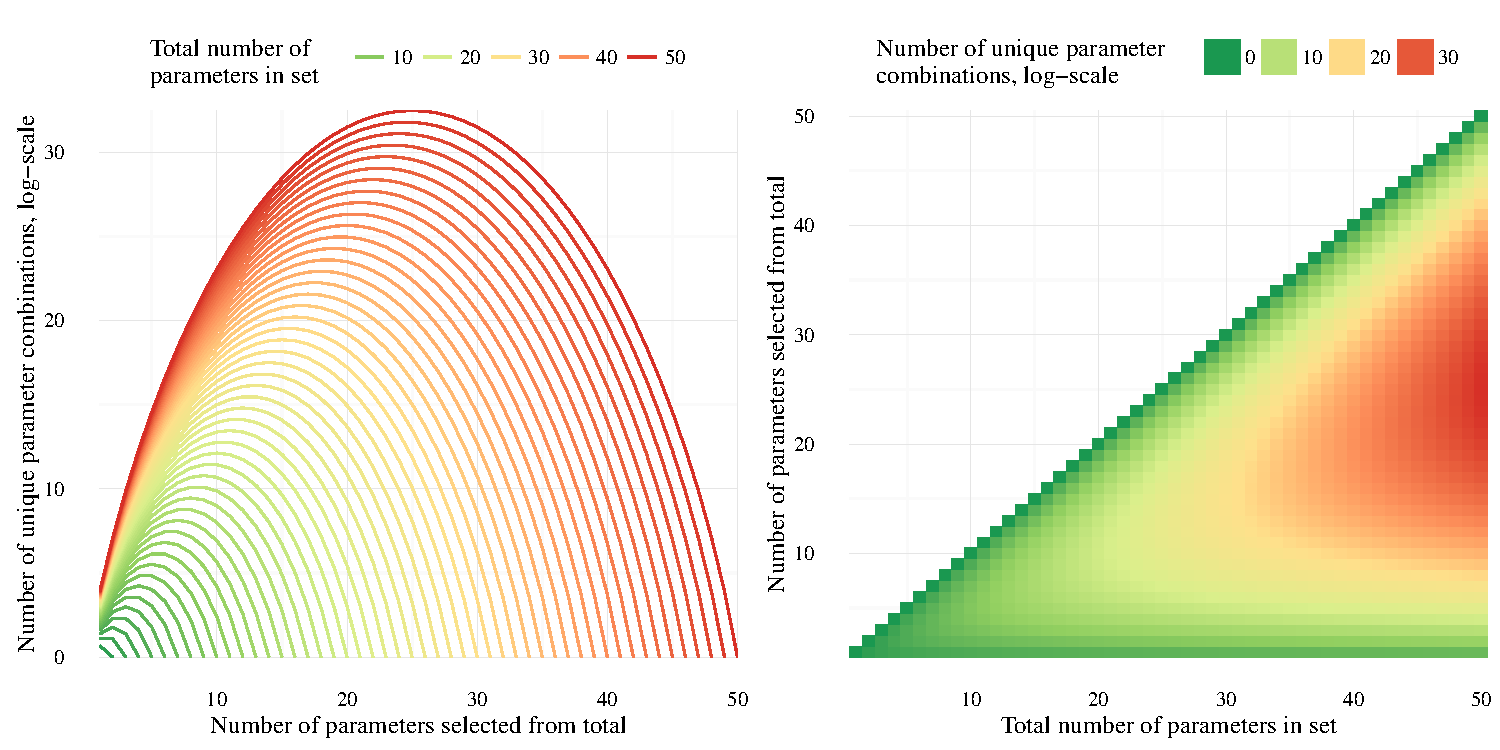
\includegraphics[width=\textwidth]{figs/unnamed-chunk-3-1} 

}

\caption[Number of unique combinations that can occur by selecting parameters for optimization from different parameter sets]{Number of unique combinations that can occur by selecting parameters for optimization from different parameter sets.  The number of combinations are shown for increasing numbers of selected parameters from the total in the set, where 100 parameter sets are shown each with one through 100 total parameters.  For example, there are six unique parameter combinations that result from choosing two parameters from a set.  Note that the number of unique combinations is shown as the natural-log.  The same information is viewed differently in each plot.}\label{fig:unnamed-chunk-3}
\end{figure}



\end{document}
